\section{Results}
\paragraph{Deployment storage.}
Table~\ref{tab:storage} reports actual saved inference-file sizes. The main 13-node deployment occupies 38,644,489 bytes versus 54,987,545 for the original model, a 29.7214\% reduction. Five nodes save a further 172,032 bytes, only a small additional reduction relative to the full original file. The measured storage improvement follows from removing the gate parameters while retaining compact FP32 lookup buffers.

\paragraph{Interpolation and table density.}
On dense P002 validation, the 13-node table's maximum signed loss is 0.000454 dB at 2.25 dB, whereas the 5-node table reaches 0.015405 dB at 2.5 dB (Fig.~\ref{fig:dense}). Both pass the predeclared tolerance. The 13-node choice offers the smaller observed loss for a modest file-size increase. On all 5,000 validation images in P003, its maximum signed loss is 0.000264 dB at 2.375 dB.

\begin{figure}[t]
 \centering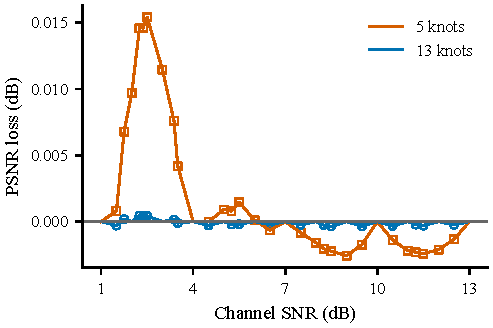
\includegraphics[width=\linewidth]{figures/dense_validation.pdf}
 \caption{Dense validation (P002): original PSNR minus table PSNR at 32 fixed SNRs, with 1,000 images and three paired noise realizations per condition. Lines guide the eye between measured points; open markers identify non-knot conditions for each table. Five-node knots are 1, 4, 7, 10, and 13 dB; 13-node knots are every integer from 1 to 13 dB. Both variants use checkpoint 21,500.}
 \label{fig:dense}
\end{figure}

\paragraph{Frozen official test.}
Table~\ref{tab:test} gives absolute reconstruction PSNR and the paired difference on the frozen test grid. The maximum signed decrease is 0.000186488 dB at 2.375 dB, with descriptive interval $[-0.0000406,0.0004124]$ dB. The maximum absolute change is 0.000337846 dB at 1.5 dB; its negative signed loss indicates a small improvement. These are different summaries of the same paired results.

Five test conditions are integer-dB table knots and show differences below $3\times10^{-8}$ dB in magnitude. The three fractional conditions, 1.5, 2.375, and 12.5 dB, exercise interpolation. Figure~\ref{fig:test} displays these differences in millidecibels so that their scale and conditional intervals remain visible. Both positive and negative differences occur, as expected for a small perturbation of a learned model rather than a monotonic quality improvement.

\begin{table}[t]
 \centering\small
 \setlength{\tabcolsep}{3pt}
\begin{tabular}{rrrrr}
\toprule
SNR & Original & 13 knots & Loss & 95\% interval \\
(dB) & (dB) & (dB) & (mdB) & (mdB) \\
\midrule
1 & 27.09260 & 27.09260 & 0.000 & [0.000, 0.000] \\
1.5 & 27.53395 & 27.53429 & -0.338 & [-0.479, -0.188] \\
2.375 & 28.27304 & 28.27285 & +0.186 & [-0.041, 0.412] \\
3 & 28.78591 & 28.78591 & 0.000 & [0.000, 0.000] \\
7 & 31.84959 & 31.84959 & 0.000 & [0.000, 0.000] \\
12 & 34.87276 & 34.87276 & 0.000 & [0.000, 0.000] \\
12.5 & 35.11328 & 35.11354 & -0.258 & [-0.269, -0.246] \\
13 & 35.33646 & 35.33646 & 0.000 & [0.000, 0.000] \\
\bottomrule
\end{tabular}

 \caption{P004 official test: 10,000 images and three paired noises at each SNR. PSNR is computed from pooled MSE. Loss is original minus 13-node PSNR, in millidecibels (mdB; $1\,\mathrm{mdB}=10^{-3}$ dB). Intervals are conditional, pointwise, and descriptive (Sec.~4). Values, including near-zero knot differences, are rounded for display.}
 \label{tab:test}
\end{table}
\begin{figure}[t]
 \centering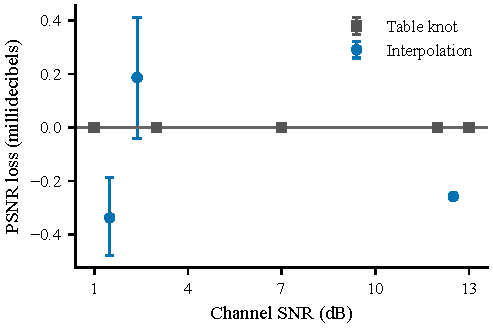
\includegraphics[width=\linewidth]{figures/frozen_test.pdf}
 \caption{Frozen P004 test differences and conditional pointwise 95\% descriptive intervals from 2,000 paired batch-cluster bootstrap draws. Each condition uses 10,000 images, three noises, and 79 batch clusters. Squares mark table knots; circles mark interpolation. Positive loss means lower PSNR for the table.}
 \label{fig:test}
\end{figure}

\paragraph{Historical controls and failure case.}
Table~\ref{tab:pilot} retains all pilot variants on their original 8,000-update checkpoint and 13-point validation grid. Linear interpolation with three knots has maximum loss 0.093756 dB; nearest-neighbor lookup with five knots has larger loss, 0.129533 dB, despite the latter's denser table. Thus, lookup resolution and interpolation rule both matter. The shared-SNR control preserves the original MLP parameters and shows a near-zero reconstruction difference, separating repeated scalar computation from parameter removal. The table values describe this historical checkpoint and grid; the dense current-checkpoint results above are a distinct experiment.

\begin{table}[t]
 \centering\small
 \begin{tabular}{lrr}
\toprule
Method & File bytes & Max. loss (dB) \\
\midrule
Original & 54,987,481 & 0.000000 \\
Shared-SNR MLP & 54,989,849 & 0.000000 \\
Linear, 3 knots & 38,429,449 & 0.093756 \\
Linear, 5 knots & 38,472,457 & 0.009071 \\
Linear, 9 knots & 38,558,473 & 0.000389 \\
Linear, 13 knots & 38,644,489 & 0.000258 \\
Nearest, 5 knots & 38,472,457 & 0.129533 \\
\bottomrule
\end{tabular}

 \caption{Historical P001 pilot: 8,000-update checkpoint, 1,000 validation images, 13 SNR conditions, three paired noises. Maximum signed loss is taken over the full recorded grid. This checkpoint is separate from Tables~\ref{tab:storage} and~\ref{tab:test}.}
 \label{tab:pilot}
\end{table}
